\documentclass{article}
\usepackage{fontspec}
\usepackage{polyglossia}
\setdefaultlanguage{french}
\usepackage[a4paper,margin=2.5cm]{geometry}

\usepackage{amsmath}
\usepackage{amssymb}
\usepackage{array}
\usepackage{auto-pst-pdf}
\usepackage{booktabs}
\usepackage{cite}
\usepackage{graphicx}
\usepackage{lmodern}
\usepackage{marvosym}
\usepackage{mathrsfs}
\usepackage{minted}
\usepackage{multicol}
\usepackage{multirow}
\usepackage{paralist}
\usepackage{schemabloc}
\usepackage{siunitx}
\usepackage{soul}
\usepackage{tikz}
\usepackage[european,cuteinductors,siunitx]{circuitikz}
\usepackage{url,hyperref}
\usepackage{verbatim}
\usepackage{xunicode,xltxtra}

\title{
\includegraphics{../../images/inp-enseeiht} \\ ~ \\ ~ \\ ~ \\ ~ \\ Initiation cadence layout (G)XL}
\author{François Pierron \& Guilhem Saurel}
\date{\oldstylenums{24 janvier 2014}}

\setlength{\columnseprule}{1pt}

\begin{document}

\begin{titlepage}
    \setcounter{page}{0}
    \maketitle
    \vfill
    \tableofcontents
    \thispagestyle{empty}
\end{titlepage}

%\section{Design and Simulation of the electrical schematic of the operational amplifier (Cadence Composer schematic editor and Spectre)}
%\section{Layout of the schematic using the technology rule sets provided by the fondery AMS for this 0.35$\mu$m CMOS process}

\section*{Introduction}

Ce TP consiste à apprendre à se servir du logiciel Cadence et des différents outils qu’il propose, tels que «Cadence Composer Schematic», «Spectre», et «Virtuoso», «Assura» et «Calibre».

Pour cela, nous allons réaliser un amplificateur opérationnel à deux étages:

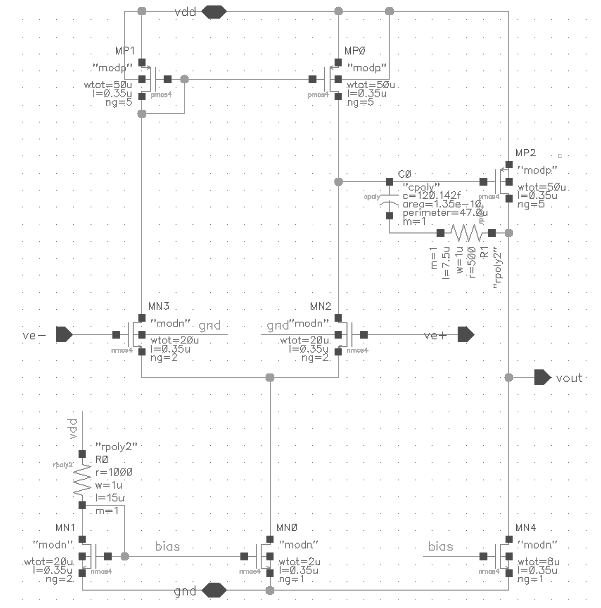
\includegraphics[width=\linewidth]{sch.png}

NB: Ce schéma est issu du sujet et pas de notre projet, vu que nous avons hiérarchisé celui-ci en diverses sous parties (charge active, miroirs de courrant, paire différentielle et source commune), et qu’on ne voit donc pas grand chose sur nos captures.

\newpage

\section{Conception et simulation du schéma électrique sous Cadence Spectre}

Pour la schématique et la simulation, à part la prise en main de la «calculette»,
il n’y a pas de grande nouveauté au passage à ce logiciel, et on obtient rapidement
un diagramme de Bode cohérent:

~

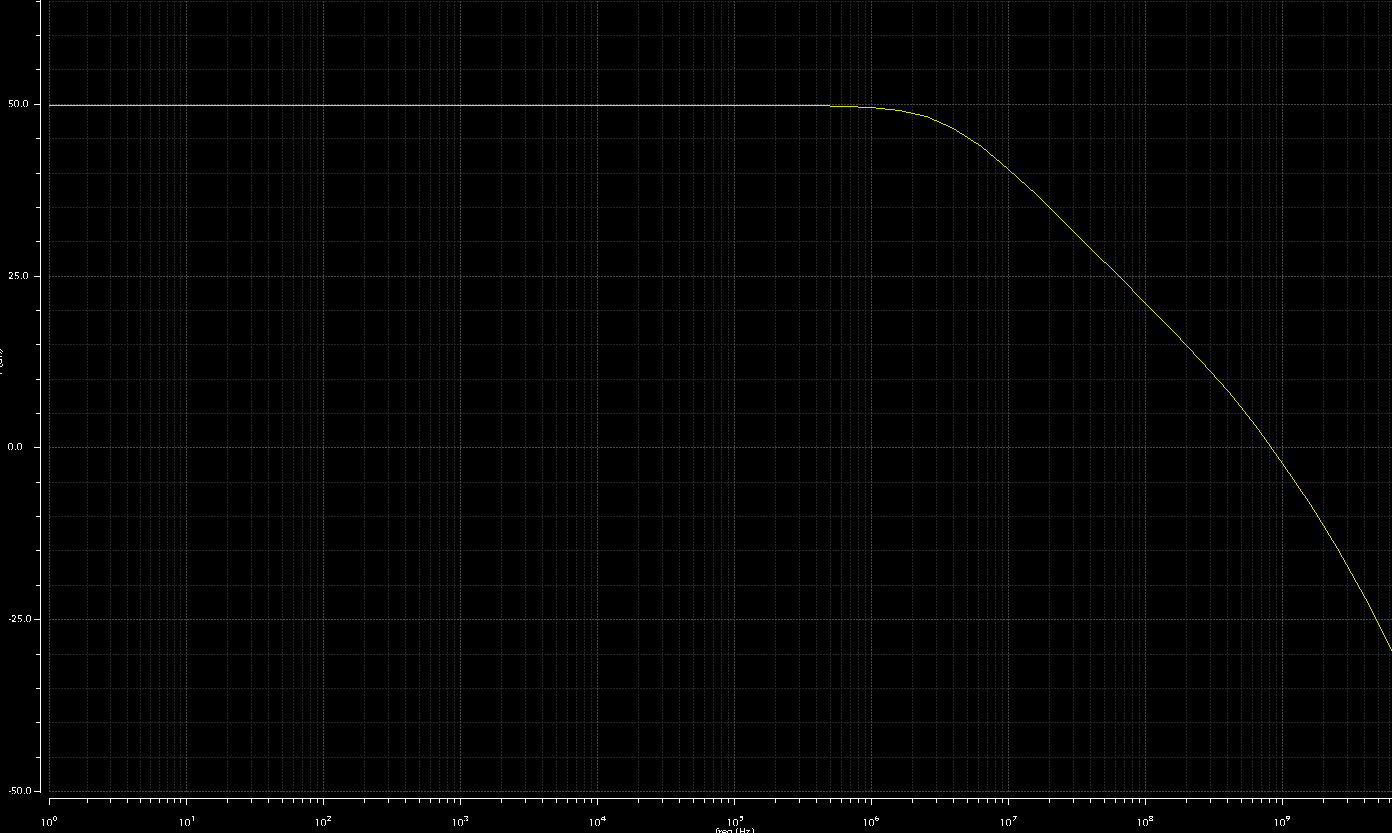
\includegraphics[width=\linewidth]{bode_sch.png}

~

Cependant, un certain nombre de paramètres sont importants à prendre en compte, puisque cette schématique va servir au layout:
\begin{itemize}
    \item Lorsqu’un transistor est trop gros, il faut augmenter le nombre de ses grilles afin qu’elles soient moins longues, et que donc la chute de potentiel dans celles-ci reste négligeable. Dans certains cas, il faudra même séparer le transistor en plusieurs parties, ce que nous avons eu besoin de faire pour le ballast dans le projet ASIC analogique.
    \item Si certains transistors travaillent de concert, il est important qu’ils aient la même taille. Pour cela, pour les transistors des miroirs de courant par exemple, au lieu d’en mettre un de 20µm, un de 2µm et un de 8µm, il faut prendre le plus petit commun multiple (2µm), et considérer que celui de 20µm est en réalité composé de 10 de 2µm, et que celui de 8µm est composé de 4 de 2µm. Sinon, il n’est pas possible de les appairer correctement, puisqu’un décalage de masque aurait un impact différent: dans cet exemple, si le masque est décalé de 0.1µm, cela affectera de 0.5\% celui de 20µm mais de 5\% celui de 2µm !
\end{itemize}

~

\newpage

\section{Layout du circuit sous Virtuoso d’après les règles CMOS AMS 0.35µm}

Notre hiérarchisation de ce circuit nous a permis de travailler en parallèle sur les diverses parties lors du routage, puis d’assembler les blocs ensemble à la fin.

\begin{multicols}{2}
    Pour la distribution des 10 + 5 + 1 transistors dans le bloc «Miroirs de courant», nous avons essayé de trouver un schéma le plus symmétrique possible qui minimiserait l’impact d’un gradient de dopage et/ou de température dans n’importe quelle direction. Nous avons commencé par opter pour un placement de ce type:

    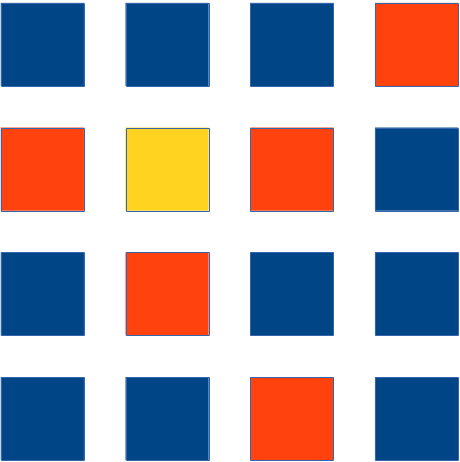
\includegraphics[width=\linewidth-1cm]{placement_mirroirs.png}


    ~

    Nous avions également envisagé une structure qui est symétrique suivant à peu près tous les axes, mais celle-ci imposait de prendre non pas 16 transistors de 2µm mais 32 de 1µm, ce qui aurait ajouté énormément de fils et nous aurions perdu en espace, sans compter la complexité et le temps nécessaire au routage:

    
\includegraphics[width=\linewidth-1cm]{placement_mirroirs_ideal.png}

    Cependant, nous nous sommes finalement rendus compte après quelques essais que nous pouvions avoir une structure encore un peu moins optimale en termes de symétrie:

    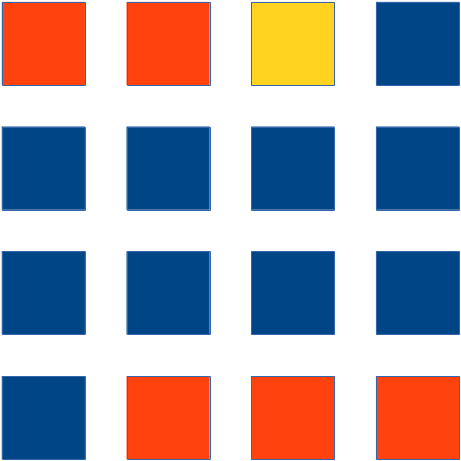
\includegraphics[width=\linewidth-1cm]{placement_mirroirs_final.png}

    ~

    Son avantage est qu’elle permet de fusionner la majorité des sources et des drains ensembles, le gain en place et en nombre de fils (et donc de capacités parasites) est alors considérable:

    ~

    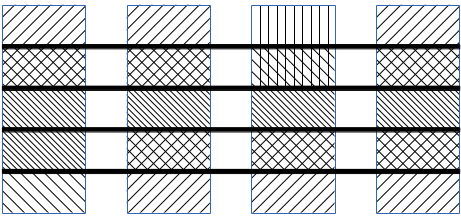
\includegraphics[width=\linewidth-1cm]{placement_mirroirs_final2.png}

    ~

    Pour les autres, paires, les transistors sont simplement placés sur les diagonales.

\end{multicols}


%~

%Une fois les différents blocs routés, il a fallu les entourer de «Guard Rings». Aucun rapport avec un quelconque livre de J.R.R. Tolkien, ces anneaux servent à créer des caissons pour isoler les transistors N du substrat P. Il faut donc les polariser à $V_{DD}$ afin que la diode engendrée soit en inverse.

%Pour arriver à faire la même chose pour les transistors P de la charge active, il faut par contre mettre un guard ring N connecté à la masse et un guard ring P connecté à $V_{DD}$

%~

%Une fois ces étapes réalisés, nous n’avions plus beaucoup de temps pour assembler le layout de niveau principal, donc il n’est peut être pas optimal, mais nous devions apprendre à effectuer les simulations post-layout, qui prennent en compte toutes les capacités parasites et les résistances des différents fils, et qui allaient nous permettre d’effectuer une comparaison avec les simulations post-schématique.

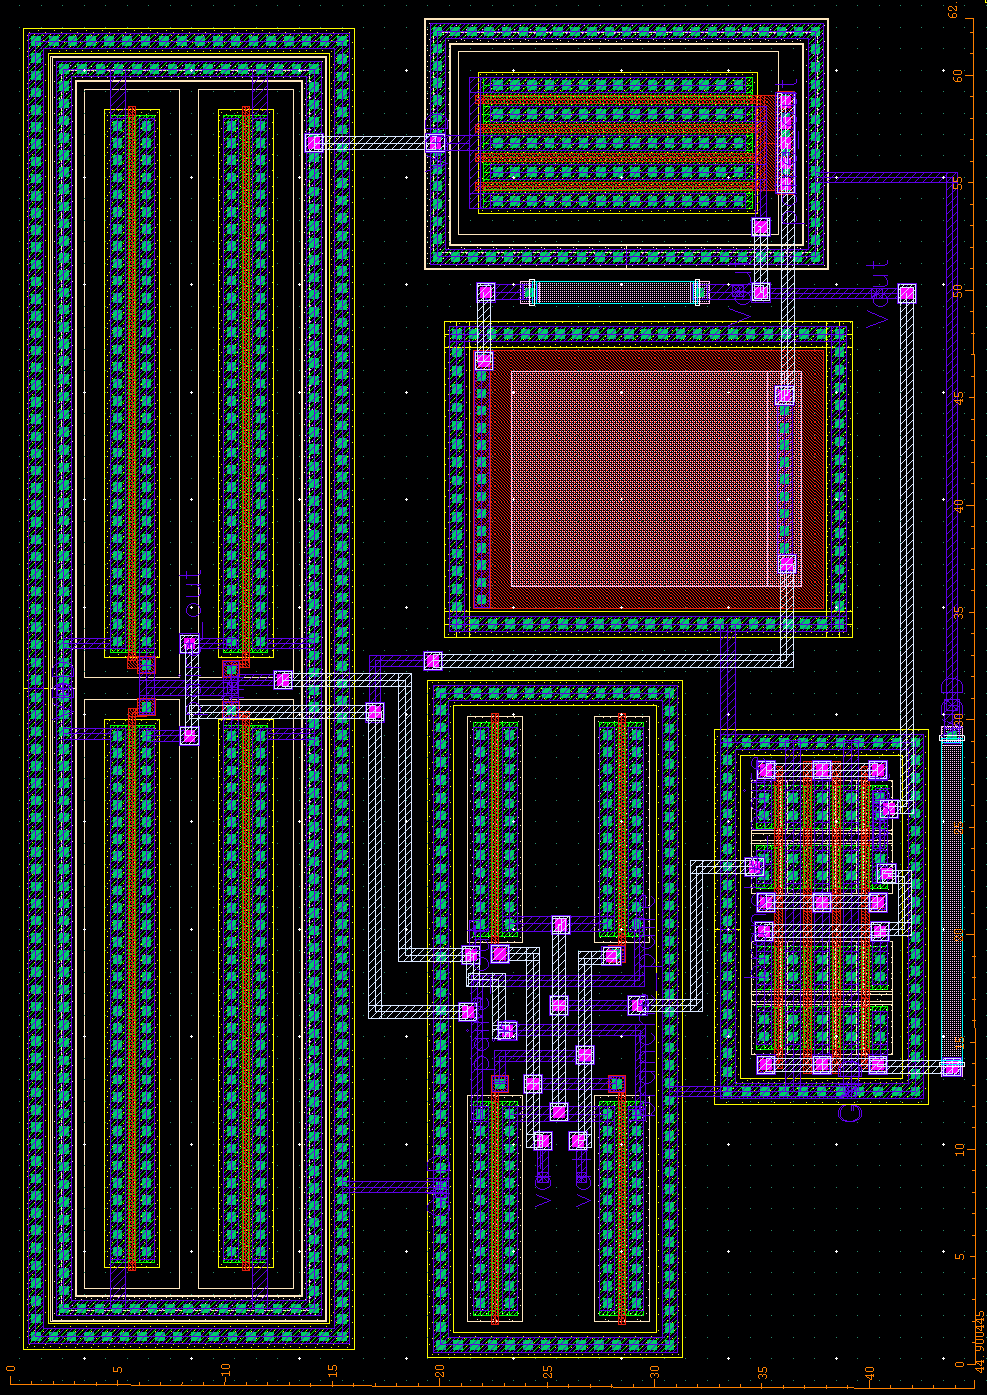
\includegraphics[width=\linewidth-0.25cm]{layout_cadence.png}

Ce design fait environ 45x63 µm.

\newpage

\section{Simulations post-layout}

%Une fois ce layout terminé, ce qui comprend des vérifications de règles de design (DRC) et le Layout Versus Schématique (LVS) (ce qui n’est pas toujours le plus rigolo ni le plus rapide), nous avons enfin pu effectuer de nouvelles simulations qui utilisaient le layout, afin de vérifier que les performances du circuit soient restées correctes, même si nous nous attendions à ce qu’elles baissent puisque nous avions inclu un bon nombre de non-idéalités.

Une fois ce layout terminé, ce qui comprend des vérifications de règles de design (DRC) et le Layout Versus Schematic (LVS) (ce qui n’est pas toujours le plus rigolo ni le plus rapide), nous avons enfin pu effectuer de nouvelles simulations qui utilisaient un modèle comportemental généré à partir du layout.

Cela permet de voir à quel point les caractéristiques du circuit idéal sont impactées par le routage : les simulations idéales ne peuvent pas prendre en compte les résistances parasites crées par les longueurs des pistes entre les transistors, les capacités qui se créent lorsque 2 pistes sont proches...

~

Nous devons nous assurer que les caractéristiques du circuit soient restées correctes, sinon nous serions obligés de revoir une partie du layout et/ou du schema pour compenser/limiter les pertes de performance.

~

\begin{tabular}{|l|r|r|}
    \hline
    Résultats & Simulation de schématique & Simulation Post-Layout \\
    \hline
    Consommation & 10.2 mW & 9.834 mW \\
    \hline
    Gain en boucle ouverte & 49 dB & 47.15 dB \\
    \hline
    Bande passante & 3.9 MHz & 4.3 MHz \\
    \hline
    Offset & 22 mV & 20mV \\
    \hline
    Input Voltage noise (Power spectrum Density) & 7mV & 6.66mV \\
    \hline
    Marge de phase & 53° & 52° \\
    \hline
    Marge de gain & 27 dB & 24.5 dB \\
    \hline
    Slew Rate & 1.155 V/ns & 1.200 V/ns \\
    \hline
\end{tabular}

Dans notre cas, les performances restent largement correctes voire s'améliorent une fois passé au modèle extrait du layout. Le plus notable est quand même la baisse du gain (~ -2dB).

%Nos résultats dans les deux simulations ne sont donc pas si différents l’un de l’autre, et ils sont même parfois légèrement supérieurs dans le cas de la simulation Post-Layout.

\section*{Conclusion}

Nous avons donc appris à nous servir de Cadence dans le but d’effectuer le design, la schématique et le layout d’un circuit, et d’en valider les différentes étapes. L’étape suivante étant la conception du procesus technologique menant du layout à la création des masques et au reste de la fabrication, que nous avons effectué lors de notre semaine en salle blanche, nous avons désormais vu la totalité des étapes nécéssaires pour obtenir un circuit électronique, ce qui est une réelle satisfaction.

\end{document}
